\begin{frame}{Featureless Insulators}
\vskip-1.5cm
\begin{columns}[T]
    \begin{column}[T]{.6\textwidth}
        \begin{block}{Definition of 'Featureless Insulator'}
            \vskip-1em
            \begin{itemize}
            \item Gapped
            \item Symmetric
            \item No (bulk) fractionalization
            \item Unique ground state on torus
            \end{itemize}
        \end{block}
        
   Examples:
    \end{column}
    \begin{column}[T]{.4\textwidth}
    \begin{figure}[h]
            \centering
            \scalebox{0.7}{
            %
% x=3*(minimum size)/2
% y=\sqrt{3/4}*(minimum size)/2
%

%http://tex.stackexchange.com/questions/6019/drawing-hexagons
\begin{tikzpicture}[x=7.5mm,y=4.33mm]
  % some styles
  \tikzset{
    box/.style={
      regular polygon,
      regular polygon sides=6,
      minimum size=10mm,
      inner sep=0mm,
      outer sep=0mm,
      rotate=0,
    draw
    }
  }
 \tikzset{boson/.style={circle=1pt,draw=black!100,fill=orange!100,inner sep=2pt}}

\foreach \i in {0,...,2} 
    \foreach \j in {0,...,3} {
            \node[box] at (2*\i,2*\j) {};
        }
\foreach \i in {0,...,1} 
    \foreach \j in {0,...,2} {
   	   \node[box] at (2*\i+1,2*\j+1) {};   
        }
\foreach \i in {0,...,2} 
    \foreach \j in {0,...,3} {
            \node[boson] at (2*\i-0.6,2*\j) {};
            \node[boson] at (2*\i+0.6,2*\j) {};
            \node[boson] at (2*\i-0.4,2*\j-1) {};
            \node[boson] at (2*\i-0.4,2*\j+1) {};
             \node[boson] at (2*\i+0.4,2*\j+1) {};
              \node[boson] at (2*\i+0.4,2*\j-1) {};
        }
%\foreach \i in {0,...,1} 
  %  \foreach \j in {0,...,2} {
%	\node[boson] at (2*\i+1-0.6,2*\j+1) {}; 
%	\node[boson] at (2*\i+1+0.6,2*\j+1) {};   
   %   }
      
\end{tikzpicture}

            }
            \caption{\begin{tabular}[t]{l}
                     Bosonic Mott insulator \\
                     with integer filling \end{tabular}}
    \end{figure}
    \end{column}
\end{columns}

\begin{columns}[T]
    \begin{column}[T]{.4\textwidth}
        \vskip-0.5cm
        \begin{figure}[h]
            \captionsetup{justification=centering}
            \centering
            \scalebox{0.6}{
             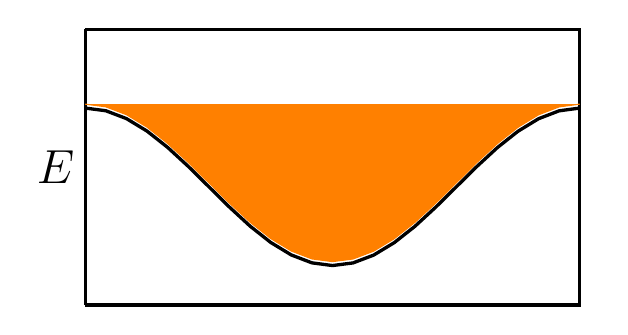
\begin{tikzpicture}[domain=0:6.28]
      \draw[very thick] (0, -2.5) -- (0,1) node[left, midway] {\LARGE $E$} ;
      \draw[very thick] (0, 1)-- (6.28,1) -- (6.28, -2.5) -- (0, -2.5);
      \draw[color=black, very thick] plot (\x,{-1+cos(\x r)}) node[right] {};
      \draw[color=orange, fill] plot (\x,{-0.95+cos(\x r)}) {};
  \end{tikzpicture}
  
            }
        \caption{Band Insulator}
        \end{figure}
    \end{column}
    \begin{column}[T]{.6\textwidth}
        \begin{figure}[h]
            \captionsetup{justification=centering}
            \scalebox{1.4}{
            \begin{frame}{MPS Example: AKLT State}
\vskip-1.5cm
\begin{block}{Haldane Phase for Spin-1 chains $(j=1, m=0)$}
\vskip-0.8cm
$$
H_{AKLT} = \sum\limits_{i} J \vec{S}_i\cdot \vec{S}_{i+1} + J' (\vec{S}_i\cdot \vec{S}_{i+1})^2 + D (S^z_i)^2+BS^x
$$
\end{block}
\begin{columns}[T]
    \begin{column}[T]{.45\textwidth}
        \vskip-1.2cm
        \begin{figure}
        \centering
        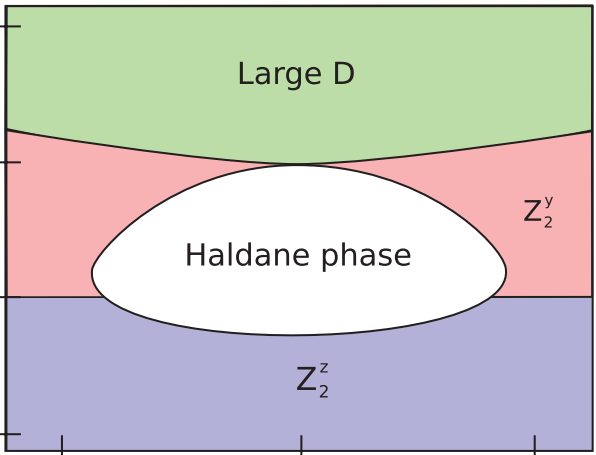
\includegraphics[width=\columnwidth]{diagrams/aklt2.png}
        \end{figure}
    \end{column}
    \begin{column}[T]{.55\textwidth}
    \vskip-0.8cm
    Two distinct featureless insulators:
    \bi 
    \item Large-D phase
    \bi 
    \item Contains product state wavefunction $\ket{\psi} = \ket{000...}$ 
    \ei
    \item Haldane phase
    \bi 
    \item Contains AKLT wavefunction $\ket{\psi} = \Sigma\ket{+00-0+...}$
    \ei 
        \begin{figure}[h]
            \hspace{-2cm}
            \scalebox{1.2}{
            \begin{frame}{MPS Example: AKLT State}
\vskip-1.5cm
\begin{block}{Haldane Phase for Spin-1 chains $(j=1, m=0)$}
\vskip-0.8cm
$$
H_{AKLT} = \sum\limits_{i} J \vec{S}_i\cdot \vec{S}_{i+1} + J' (\vec{S}_i\cdot \vec{S}_{i+1})^2 + D (S^z_i)^2+BS^x
$$
\end{block}
\begin{columns}[T]
    \begin{column}[T]{.45\textwidth}
        \vskip-1.2cm
        \begin{figure}
        \centering
        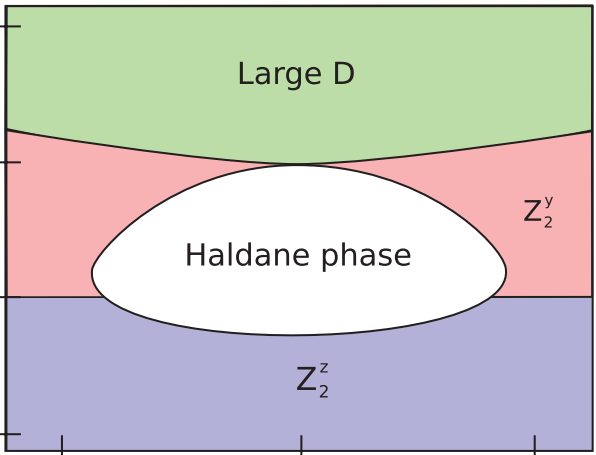
\includegraphics[width=\columnwidth]{diagrams/aklt2.png}
        \end{figure}
    \end{column}
    \begin{column}[T]{.55\textwidth}
    \vskip-0.8cm
    Two distinct featureless insulators:
    \bi 
    \item Large-D phase
    \bi 
    \item Contains product state wavefunction $\ket{\psi} = \ket{000...}$ 
    \ei
    \item Haldane phase
    \bi 
    \item Contains AKLT wavefunction $\ket{\psi} = \Sigma\ket{+00-0+...}$
    \ei 
        \begin{figure}[h]
            \hspace{-2cm}
            \scalebox{1.2}{
            \begin{frame}{MPS Example: AKLT State}
\vskip-1.5cm
\begin{block}{Haldane Phase for Spin-1 chains $(j=1, m=0)$}
\vskip-0.8cm
$$
H_{AKLT} = \sum\limits_{i} J \vec{S}_i\cdot \vec{S}_{i+1} + J' (\vec{S}_i\cdot \vec{S}_{i+1})^2 + D (S^z_i)^2+BS^x
$$
\end{block}
\begin{columns}[T]
    \begin{column}[T]{.45\textwidth}
        \vskip-1.2cm
        \begin{figure}
        \centering
        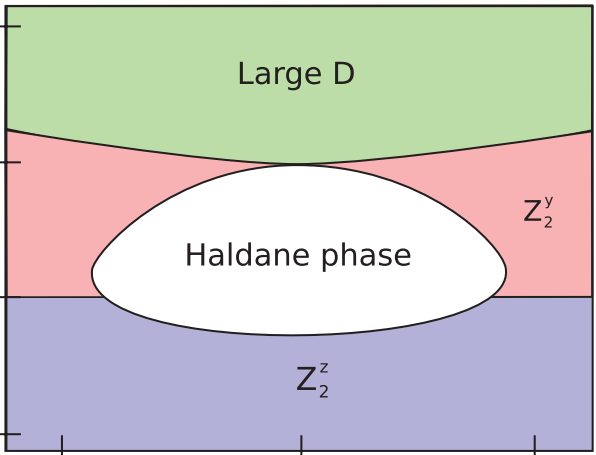
\includegraphics[width=\columnwidth]{diagrams/aklt2.png}
        \end{figure}
    \end{column}
    \begin{column}[T]{.55\textwidth}
    \vskip-0.8cm
    Two distinct featureless insulators:
    \bi 
    \item Large-D phase
    \bi 
    \item Contains product state wavefunction $\ket{\psi} = \ket{000...}$ 
    \ei
    \item Haldane phase
    \bi 
    \item Contains AKLT wavefunction $\ket{\psi} = \Sigma\ket{+00-0+...}$
    \ei 
        \begin{figure}[h]
            \hspace{-2cm}
            \scalebox{1.2}{
            \input{diagrams/aklt.tex}
            }
        \end{figure}

    \ei
    \end{column}
\end{columns}

\end{frame}
            }
        \end{figure}

    \ei
    \end{column}
\end{columns}

\end{frame}
            }
        \end{figure}

    \ei
    \end{column}
\end{columns}

\end{frame}
            }
            \caption{Haldane phase of spin-1 Chain (AKLT)}
        \end{figure}
    \end{column}
\end{columns}
\end{frame}